Um die zuvor erwähnte Theorie nachzuweisen kann der Aufbau aus Abb. \ref{fig:aufbau}
verwendet werden.
\begin{figure}
  \centering
  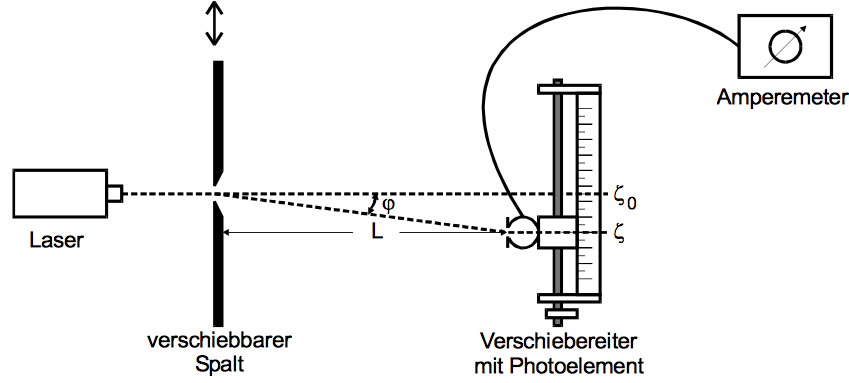
\includegraphics[width=0.8\textwidth]{bilder/aufbau.png}
  \caption{Versuchsaufbau für Beugungsexperimente \cite{406}}
  \label{fig:aufbau}
\end{figure}
Ein He-Ne-Laser der Wellenlänge $\lambda = 633 \,\si{\nano\meter}$ bestrahlt
einen Spalt der Spaltbreite $b = (20-200) \,\si{\micro\meter}$. Im Abstand von
$(100-120) \cm$ ist ein Detektor aufgestellt, der mit einer Photodiode das
Beugungsbild aufnimmt. Zur Messung dient ein Messverschiebereiter senkrecht zur
optischen Achse. Da die Photodiode auch einen thermischen Dunkelstrom $I_\su{du}$
misst, muss dieser Dunkelstrom zuvor bei abgedeckter Blende gemessen werden, um ihn
später bei den Messergebnissen wieder abziehen zu können.

Der Detektor wird in der Mittelstellung des Messverschiebereiters fixiert und nur
die Spaltblende wird so lange justiert, bis die n-ten Nebenmaxima links und rechts
vom Hauptmaximum in etwa die gleiche Intensität haben.
Die Intensität $I(\zeta)$ wird dann in Abhängigkeit der Detektorstellung $\zeta$
punktweise gemessen. Die Detektorstellung kann in $\si{\milli\meter}$ auf der
Detektorskala abgelesen werden. Eine Trommelumdrehung entspricht $1\,\si{\milli\meter}$,
ein Teilstrich auf der Trommel entsprechen $10\,\si{\micro\meter}$.
Um später das gemessene $I(\zeta)$ mit dem berechneten $I(\varphi)$ zu vergleichen,
wird der Beugungswinkel näherungsweise durch
\begin{equation}
  \varphi \approx \tan{(\varphi)} = \frac{\zeta - \zeta_0}{L}
\end{equation}
bestimmt. $\zeta_0$ meint die Ausgangsstellung des Verschiebereiters,also wenn der
Lichtstrahl ungebeugt ist,
und $L$ ist der Abstand zwischen Beugungsplatte und Detektorblende.

Für Einzelspalt und Doppelspalt wird analog vorgegangen.

Da in diesem Experiment auch ein Mikroskop zur Messung der Spaltbreite verwendet
wird, muss dieses vorher geeicht werden. Dazu wird ein Objektmikrometer auf den
Objekttisch gelegt und die lineare Skala wird dann auf $\si{\micro\meter}$ geeicht,
indem die beiden Skalen miteinander verglichen werden. Ein Teilstrich entspricht
$10\,\si{\micro\meter}$.
